
\documentclass[journal,12pt,twocolumn]{IEEEtran}

\usepackage{setspace}
\usepackage{gensymb}
\singlespacing
\usepackage[cmex10]{amsmath}
\usepackage{amssymb}
\usepackage{xurl}

\usepackage{amsthm}
\usepackage{comment}
\usepackage{mathrsfs}
\usepackage{txfonts}
\usepackage{stfloats}
\usepackage{bm}
\usepackage{cite}
\usepackage{cases}
\usepackage{subfig}

\usepackage{longtable}
\usepackage{multirow}

\usepackage{enumitem}
\usepackage{mathtools}
\usepackage{steinmetz}
\usepackage{tikz}
\usepackage{circuitikz}
\usepackage{verbatim}
\usepackage{tfrupee}
\usepackage[breaklinks=true]{hyperref}
\usepackage{graphicx}
\usepackage{tkz-euclide}

\usetikzlibrary{calc,math}
\usepackage{listings}
    \usepackage{color}                                            %%
    \usepackage{array}                                            %%
    \usepackage{longtable}                                        %%
    \usepackage{calc}                                             %%
    \usepackage{multirow}                                         %%
    \usepackage{hhline}                                           %%
    \usepackage{ifthen}                                           %%
    \usepackage{lscape}     
\usepackage{multicol}
\usepackage{chngcntr}

\DeclareMathOperator*{\Res}{Res}

\renewcommand\thesection{\arabic{section}}
\renewcommand\thesubsection{\thesection.\arabic{subsection}}
\renewcommand\thesubsubsection{\thesubsection.\arabic{subsubsection}}

\renewcommand\thesectiondis{\arabic{section}}
\renewcommand\thesubsectiondis{\thesectiondis.\arabic{subsection}}
\renewcommand\thesubsubsectiondis{\thesubsectiondis.\arabic{subsubsection}}


\hyphenation{op-tical net-works semi-conduc-tor}
\def\inputGnumericTable{}                                 %%

\lstset{
%language=C,
frame=single, 
breaklines=true,
columns=fullflexible
}
\begin{document}


\newtheorem{theorem}{Theorem}[section]
\newtheorem{problem}{Problem}
\newtheorem{proposition}{Proposition}[section]
\newtheorem{lemma}{Lemma}[section]
\newtheorem{corollary}[theorem]{Corollary}
\newtheorem{example}{Example}[section]
\newtheorem{definition}[problem]{Definition}

\newcommand{\BEQA}{\begin{eqnarray}}
\newcommand{\EEQA}{\end{eqnarray}}
\newcommand{\define}{\stackrel{\triangle}{=}}
\bibliographystyle{IEEEtran}
\raggedbottom
\setlength{\parindent}{0pt}
\providecommand{\mbf}{\mathbf}
\providecommand{\pr}[1]{\ensuremath{\Pr\left(#1\right)}}
\providecommand{\qfunc}[1]{\ensuremath{Q\left(#1\right)}}
\providecommand{\sbrak}[1]{\ensuremath{{}\left[#1\right]}}
\providecommand{\lsbrak}[1]{\ensuremath{{}\left[#1\right.}}
\providecommand{\rsbrak}[1]{\ensuremath{{}\left.#1\right]}}
\providecommand{\brak}[1]{\ensuremath{\left(#1\right)}}
\providecommand{\lbrak}[1]{\ensuremath{\left(#1\right.}}
\providecommand{\rbrak}[1]{\ensuremath{\left.#1\right)}}
\providecommand{\cbrak}[1]{\ensuremath{\left\{#1\right\}}}
\providecommand{\lcbrak}[1]{\ensuremath{\left\{#1\right.}}
\providecommand{\rcbrak}[1]{\ensuremath{\left.#1\right\}}}
\theoremstyle{remark}
\newtheorem{rem}{Remark}
\newcommand{\sgn}{\mathop{\mathrm{sgn}}}
\providecommand{\abs}[1]{\vert#1\vert}
\providecommand{\res}[1]{\Res\displaylimits_{#1}} 
\providecommand{\norm}[1]{\lVert#1\rVert}
%\providecommand{\norm}[1]{\lVert#1\rVert}
\providecommand{\mtx}[1]{\mathbf{#1}}
\providecommand{\mean}[1]{E[ #1 ]}
\providecommand{\fourier}{\overset{\mathcal{F}}{ \rightleftharpoons}}
%\providecommand{\hilbert}{\overset{\mathcal{H}}{ \rightleftharpoons}}
\providecommand{\system}{\overset{\mathcal{H}}{ \longleftrightarrow}}
	%\newcommand{\solution}[2]{\textbf{Solution:}{#1}}
\newcommand{\solution}{\noindent \textbf{Solution: }}
\newcommand{\cosec}{\,\text{cosec}\,}
\providecommand{\dec}[2]{\ensuremath{\overset{#1}{\underset{#2}{\gtrless}}}}
\newcommand{\myvec}[1]{\ensuremath{\begin{pmatrix}#1\end{pmatrix}}}
\newcommand{\mydet}[1]{\ensuremath{\begin{vmatrix}#1\end{vmatrix}}}
\numberwithin{equation}{subsection}
\makeatletter
\@addtoreset{figure}{problem}
\makeatother
\let\StandardTheFigure\thefigure
\let\vec\mathbf
\renewcommand{\thefigure}{\theproblem}
\def\putbox#1#2#3{\makebox[0in][l]{\makebox[#1][l]{}\raisebox{\baselineskip}[0in][0in]{\raisebox{#2}[0in][0in]{#3}}}}
     \def\rightbox#1{\makebox[0in][r]{#1}}
     \def\centbox#1{\makebox[0in]{#1}}
     \def\topbox#1{\raisebox{-\baselineskip}[0in][0in]{#1}}
     \def\midbox#1{\raisebox{-0.5\baselineskip}[0in][0in]{#1}}
\vspace{3cm}
\title{AI1103 : Assignment 3}
\author{Savarana Datta - AI20BTECH11008}
\maketitle
\newpage
\bigskip
\renewcommand{\thefigure}{\theenumi}
\renewcommand{\thetable}{\theenumi}
Download all python codes from 
\begin{lstlisting}
https://github.com/SavaranaDatta/AI1103/tree/main/Assignment3/codes
\end{lstlisting}
%
and latex codes from 
%
\begin{lstlisting}
https://github.com/SavaranaDatta/AI1103/blob/main/Assignment3/Assignment3.tex
\end{lstlisting}


\section*{Problem(GATE 1996(MA) 25)}
Let $Y_{1},Y_{2},...,Y_{15}$ be a random sample of size 15 from the probability density function \\
$f_{y}(y)=3(1-y)^{2} , 0<y<1$\\
Use the central limit theorem to approximate $P\brak{\frac{1}{8}<\Bar{Y}<\frac{3}{8}}$
\section*{Solution(GATE 1996(MA) 25)}
The \textbf{central limit theorem} states that whenever a random sample of size n is taken from any distribution with mean and variance, then the sample mean will be approximately normally distributed with mean and variance. The larger the value of the sample size, the better the approximation to the normal.
\begin{align}
\tag{1.1}
    Z_{n}=\frac{\bar{Y}-\mu}{\frac{\sigma}{\sqrt{n}}}
    \label{eq:1}
\end{align}
From equation \ref{eq:1}
\begin{align}
    \tag{1.2}
    \bar{Y}=Z_{n}\brak{\frac{\sigma}{\sqrt{n}}}+\mu
\end{align}
\begin{align}
\tag{1.3}
\pr{\frac{1}{8}<\Bar{Y}<\frac{3}{8}}
&=\pr{\frac{1}{8}<Z_{n}\brak{\frac{\sigma}{\sqrt{n}}}+\mu<\frac{3}{8}}\\
\tag{1.4}  
&=\pr{\frac{\frac{1}{8}-\mu}{\frac{\sigma}{\sqrt{n}}}<Z_{n}<\frac{\frac{3}{8}-\mu}{\frac{\sigma}{\sqrt{n}}}}
\label{eq;123}
\end{align}
$\bar{Y}$:Mean of the randomly selected 15 variables
\begin{align}
\tag{1.5}
    \bar{Y}=\frac{Y_{1}+Y_{2}+..Y_{15}}{15}
\end{align}
Mean of probability density function is
\begin{align}
\tag{1.6}
\mu&=\int_{-\infty}^{\infty}yf(y)dy\\
\tag{1.7}
    &=\int_{0}^{1}y\times 3(1-y)^{2}dy\\
\tag{1.8}
    &=\frac{1}{4}
\end{align}
Variance of probability density function is
\begin{align}
\tag{1.9}
\sigma^{2}&=E[y^{2}]-(E[y])^{2}\\
\tag{1.10}
\label{eq;2}
      &=\brak{\int_{0}^{1}y^{2}f(y)dy} - \brak{\frac{1}{4}}^{2}
\end{align}
\begin{align}
\tag{1.11}
    \int_{0}^{1}y^{2}f(y)dy &= \int_{0}^{1}y^{2}\times3(1-y)^{2}dy\\
\tag{1.12}
                            &=3\int_{0}^{1}(y-y^{2})^{2}dy\\
\tag{1.13}
\label{eq;3}
                            &=\frac{1}{10}
\end{align}
Substituting equation \ref{eq;3} in equation \ref{eq;2}
\begin{align}
\tag{1.14}
 \sigma^{2}&=\frac{1}{10}-\frac{1}{16}\\
\tag{1.15}
           &=\frac{3}{80}
\end{align}
\begin{figure}[ht]
    \centering
    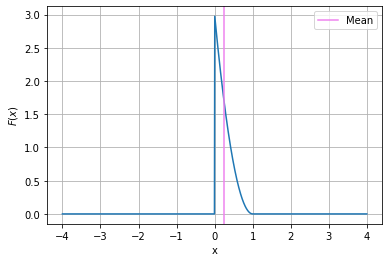
\includegraphics[width=\columnwidth]{Fig_1.png}
    \caption{}
    \label{Fig_1}
\end{figure}\\
Using Q function in equation \ref{eq;123} we have,
\begin{align}
\notag
\pr{\frac{1}{8}<\Bar{Y}<\frac{3}{8}}
&=\pr{\frac{\frac{1}{8}-\mu}{\frac{\sigma}{\sqrt{n}}}<Z_{n}<\frac{\frac{3}{8}-\mu}{\frac{\sigma}{\sqrt{n}}}}\\
\tag{1.16}
&=\pr{\frac{\frac{1}{8}-\mu(y)}{\frac{\sigma}{\sqrt{n}}}<Z_{n}<\frac{\frac{3}{8}-\mu(y)}{\frac{\sigma}{\sqrt{n}}}}\\
\tag{1.17}
&=Q\brak{\frac{\frac{-1}{8}}{\sqrt{\frac{3}{80}}}}-Q\brak{\frac{\frac{1}{8}}{\sqrt{\frac{3}{80}}}}\\
\tag{1.18}
&=1-2Q\brak{\frac{\frac{1}{8}}{\sqrt{\frac{3}{80}}}}\\
\tag{1.19}                             
&=1-2Q\brak{0.645}\\
\tag{1.20}                             
&=0.9938
\end{align}
\begin{figure}[ht]
    \centering
    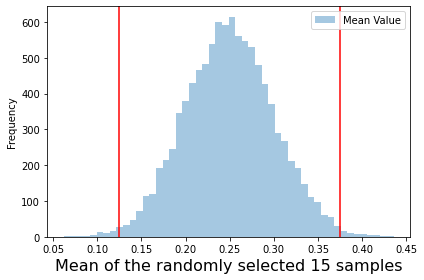
\includegraphics[width=\columnwidth]{Fig_2.png}
    \caption{}
    \label{Fig_2}
\end{figure}
\end{document}